% Szglab4
% ===========================================================================
%
\chapter{Követelmény, projekt, funkcionalitás}

\thispagestyle{fancy}

\section{Bevezetés}

\subsection{Cél}

%\comment{A dokumentum célja.}
Ez a dokumentum egy szoftverfejlesztési projekt információit tartalmazza az ötlettől a kész termékig, minden lépést naplózva. A projekt a simon\_balazst\_szeretnenk\_konzulensnek csapat által a Jégmező nevű játék fejlesztése.

\subsection{Szakterület}

%\comment{A kialakítandó szoftver milyen területen használható, milyen célra.}
A feladat játékprogram készítése, melyben a játékosok legalább háromfős csapatban működnek együtt. A program személyi számítógépeken, grafikus módban fog futni. A játék offline, tehát a több játékos egy számítógépen játssza. 

\subsection{Definíciók, rövidítések}
%\comment{A dokumentumban használt definíciók, rövidítések magyarázata.}
Még nincs.

\subsection{Hivatkozások}
%\comment{A dokumentumban használt anyagok, web-oldalak felsorolása}
Még nincs.

\subsection{Összefoglalás}
% TODO: összefoglalás

Ez a dokumentum a projekt megtervezésének és fejlesztésének tervét, valamint a projekt által meghatározott követelményeknek a listáját tartalmazza.
\begin{itemize}
\item Az áttekintés (2.2) részben tárgyaljuk a program részletesebb leírását, a felhasználók tulajdonságait, melyet szem előtt tartva folytatjuk a szoftver tervezését, fejlesztését.
\item A követelmények (2.3) rész tartalmazza a követelmények kidolgozását, melyeket a fejlesztés során majd teljesíteni kell, és ami a feladat elvárt megoldásához elengedhetetlen.
\item A Use-case leírások (2.4) tartalmazzák azokat az interakciókat, melyek a szoftverben megjelennek, vagy felhasználó, vagy belső aktorok által, a játék menetét irányítva.
\item A szótár (2.5) a fejlesztés és a program használata során megjelenő alapvető fogalmakat tartalmazza.
\item A projekt terv (2.6) a határidőkre lebontott terve, valamint a csapattagok közötti feladat kiosztás, illetve a projektvezetés menete.
\end{itemize}
\section{Áttekintés}
\subsection{Általános áttekintés}
%\comment{A kialakítandó szoftver legmagasabb szintű architekturális képe. A fontosabb alrendszerek felsorolása, a közöttük kialakítandó interfészek lényege, a felhasználói kapcsolatok alapja. Esetleges hálózati és adattárolási elvárások.}
A szoftver három fő komponense a Model, a View, és a Controller. A Model reprezentálja a játék állapotát. A View kapcsolódik a Modelhez, és megjeleníti azt. A Controller felelős a felhasználói bemenetek kezeléséért és a Model frissítéséért. Ez ismertebb nevén az MVC architektúra.

\subsection{Funkciók}
%\comment{A feladat kb. 4000 karakteres (kb 1,5 oldal) részletezettségű magyar nyelvű leírása. Nem szerepelhetnek informatikai kifejezések.}
\begin{itemize}
\item A játékban a különböző képességű szereplőknek (3 vagy több játékos lehet) kell egy tengerrel körülvett jégmezőn túlélniük. A szereplők lehetnek eszkimók vagy sarkkutatók, és körökre osztva tevékenykednek.

\item A jégmező jégtáblákból áll. Vannak stabil jégtáblák, amelyeken akárhány szereplő állhat, és vannak instabil jégtáblák, amik adott létszám felett átfordulnak és ilyenkor a rajtuk állók a vízbe esnek. A jégtáblákat a játék kezdetén eltérő mennyiségű hó borítja.

\item Az egyes jégtáblákba különféle tárgyak lehetnek belefagyva: lapát, kötél, búvárruha, élelem, stb. Befagyott tárgyat csak akkor lehet meglátni és kiásni, ha a jégtábla tiszta, nem borítja hó. A jégtáblák között lehetnek hóval fedett lukak is, amibe beleesve csak a búvárruhát viselők élnek túl, vagy azok, akiket egy köteles barátjuk a szomszéd jégtábláról azonnal kimenekít.

\item Minden szereplő egy körben 4 egységnyi munkát végezhet. Ilyen munka például a jégtáblán levő egységnyi mennyiségű hó eltakarítása, egy szomszédos jégtáblára való lépés vagy egy kiásott tárgy felvétele. A lapáttal két egységnyi hó takarítható el egy munkaráfordítással.

\item A jégmezőn időnként feltámad a hóvihar, és néhány érintett jégtáblát újabb adag friss hóval borít be. Akit elkap, annak a testhője egységnyivel csökken. Az eszkimóknak a játék elején 5 egység testhője van, a sarkkutatónak csak 4. Egy élelem eggyel növeli a testhőt.

\item A szereplők jégtábláról-jégtáblára haladnak képességeiknek megfelelően. A sarkkutató meg tudja nézni, hogy az a jégtábla, amire lépne, hány embert bír el (a luk egyet sem). Az eszkimó tud iglut építeni, amiben átvészelhetők a hóviharok. Egy-egy képesség alkalmazása is egy-egy munkát jelent.

\item A játék célja egy jelzőrakéta alkatrészeinek (pisztoly, jelzőfény, patron) megtalálása. Az alkatrészek is a jégbe vannak fagyva. Ha ezeket a csapat összegyűjti és ugyanarra a jégtáblára viszi, akkor egy munka felhasználásával összeszerelhetik és elsüthetik, amivel megnyerik a játékot. Ehhez azonban mindannyiuknak ugyanott kell állniuk. Ha valaki menet közben meghal (vízbe esve megfullad vagy elfogy a testhője és kihűl), akkor a játék véget ér. 

\item A játék felülnézetes, 2 dimenziós, a jégtáblákon lévő hó magasságát a grafikával fogjuk érzékeltetni. A jégtáblák ugyanakkora méretűek, az alakjuk még nem tisztázott, viszont ami biztos, hogy teljesen lefedik a pályát, azaz egy olyan alakzat lesz, ami képes a teljes sík tesszellációjára.
\end{itemize}

\subsection{Felhasználók}
\begin{itemize}
\item A szoftver felhasználói a szereplőket irányító játékosok, a szoftver által megadott módon irányítják avatárjaikat a játék szabályai szerint.

\item A felhasználók csak a játék szabályait ismerik, egyéb előzetes tudásuk nincs.

\item A felhasználók a program instrukciói alapján irányítják a szereplőket.

\item Legalább 3 játékosra van szükség a játék elkezdéséhez.
\end{itemize}

\subsection{Korlátozások}
% TODO: korlátozások (nemfunkcionális követelmények alapján)
\begin{itemize}
	\item A szoftver az elvárásoknak megfelelően válaszol a felhasználó(k) bemeneteire.
	\item A szoftver stabilan fut, játék közben reagál a játékosokra (nem fagy le).
\end{itemize}

\subsection{Feltételezések, kapcsolatok}
%\comment{A dokumentumban használt anyagok, web-oldalak felsorolása}
Még nincs.

\section{Követelmények}
\subsection{Funkcionális követelmények}


%\comment{Az alábbi táblázat kitöltésével készítendő. Dolgozzon ki követelmény azonosító rendszert! Az ellenőrzés módja szokásosan bemutatás és/vagy kiértékelés. Prioritás lehet alapvető, fontos, opcionális. Az alapvető követelmények nem teljesítése végzetes. Forrás alatt a követelményt előíró anyagot, szervezetet kell érteni. Esetünkben forrás lehet maga a csapat is, mikor ő talál ki követelményt. Use-case-ek alatt az adott követelményt megvalósító használati esete(ke)t kell megadni.}
% TODO: funkcionális követelmények

% Azonosító, Leírás, Ellenőrzés, Prioritás, Forrás, Use-case, Komment
\begin{longtable}{| l | p{4cm} | l | l | l | p{2cm} | l |}
\hline
\textbf{Azonosító}   & \textbf{Leírás} & \textbf{Ellenőrzés} & \textbf{Prioritás} & \textbf{Forrás} & \textbf{Use-case} & \textbf{Komment} \tabularnewline
\hline\hline
R00 & A játékban a különböző képességű szereplők vannak. & bemutatás & alapvető & feladatleírás & Build igloo, Examine tile & - \tabularnewline
\hline
R01 & Nekik kell egy tengerrel körülvett jégmezőn túlélniük & bemutatás & alapvető & feladatleírás & Step, Save & - \tabularnewline
\hline
R02 & A szereplők lehetnek eszkimók vagy sarkkutatót, és körökre osztva tevékenykednek & bemutatás & alapvető & feladatleírás & Step, Dig, Pick item up, Make rocket, Build igloo, Examine tile & - \tabularnewline
\hline
R03 & A jégmező jégtáblákból áll. & bemutatás & alapvető & feladatleírás & Turn unstable ice, Examine tile, Step & - \tabularnewline
\hline
R04 & Vannak stabil jégtáblák, amelyeken akárhány szereplő állhat, és vannak instabil jégtáblák, amik adott létszám felett átfordulnak és ilyenkor a tajuk állók a vízbe esnek. & bemutatás & alapvető & feladatleírás & Turn unstable ice, Step & - \tabularnewline
\hline
R05 & A jégtáblákat a játék kezdetén eltérő mennyiségű hó borítja. & bemutatás & alapvető & feladatleírás & Dig & - \tabularnewline
\hline
R06 & Az egyes jégtáblákba különféle tárgyak lehetnek belefagyva: lapát, kötél, búvárruha, élelem, stb. & bemutatás & alapvető & feladatleírás & Dig, Pick item up & - \tabularnewline
\hline
R07 & Befagyott tárgyat csak akkor lehet meglátni és kiásni, ha a jégtábla tiszta, nem borítja hó. & bemutatás & alapvető & feladatleírás & Dig, Pick item up & - \tabularnewline
\hline
R08 & A jégtáblák között lehetnek hóval fedett lukak is, amibe beleesve csak a búvárruhát viselők élnek túl, vagy azok, akiket egy köteles barátjuk a szomszéd jégtábláról azonnal kimenekít. & bemutatás & alapvető & feladatleírás & Step, Save drowning teammate, Examine tile & - \tabularnewline
\hline
R09 & Minden szereplő egy körben 4 egységnyi munkát végezhet. Ilyen munka például a jégtáblán levő egységnyi mennyiségű hó eltakarítása, egy szomszédos jégtáblára való lépés vagy egy kiásott tárgy felvétele. & bemutatás & alapvető & feladatleírás & Step, Dig, Pick item up, Make rocket, Save drowning teammate, Examine tile, Build igloo & - \tabularnewline
\hline
R10 & A lapáttal két egységnyi hó takarítható el egy munkaráfordítással. & bemutatás & alapvető & feladatleírás & Dig & - \tabularnewline
\hline
R11 & A jégmezőn időnként feltámad a hóvihar, és néhány érintett jégtáblát újabb adag friss hóval borít be. Akit elkap, annak a testhője egységnyivel csökken & bemutatás & alapvető & feladatleírás & Create snowstorm & - \tabularnewline
\hline
R12 & Az eszkimóknak a játék elején 5 egység testhője van, a sarkkutatóknak csak 4. Egy élelem eggyel növeli a testhőt. & bemutatás & alapvető & feladatleírás & Pick item up & - \tabularnewline
\hline
R13 & A szereplők jégtábláról-jégtáblára haladnak képességeiknek megfelelően. & bemutatás & alapvető & feladatleírás  & Step & - \tabularnewline
\hline
R14 & A sarkkutató meg tudja nézni, hogy az a jégtábla, amire lépne, hány embert bír el (a luk egyet sem). & bemutatás & alapvető & feladatleírás & Examine tile & - \tabularnewline
\hline
R15 & Az eszkimó tud iglut építeni, amiben átvészelhetők a hóviharok. Egy-egy képesség alkalmazása is egy-egy munkát jelent. & bemutatás & alapvető & feladatleírás & Build igloo & - \tabularnewline
\hline
R16 & A játék célja egy jelzőrakéta alkatrészeinek (pisztoly, jelzőfény, patron) megtalálása. & bemutatás & alapvető & feladatleírás & Make rocket, Dig, Pick item up & - \tabularnewline
\hline
R17 & Az alkatrészek is a jégbe vannak fagyva. & bemutatás & alapvető & feladatleírás & Dig, Pick item up & - \tabularnewline
\hline
R18 & Ha ezeket a csapat összegyűjti és ugyanarra a jégtáblára viszi, akkor egy munka felhasználásával összeszerelhetik és elsüthetik, amivel megnyerik a játékot. Ehhez azonban mindannyiuknak ugyanott kell állniuk. & bemutatás & alapvető & feladatleírás & Make rocket & - \tabularnewline
\hline
R19 & Ha valaki menet közben meghal (vízbe esve megfullad vagy elfogy a testhője és kihűl), akkor a játék véget ér & bemutatás & alapvető & feladatleírás & Turn unstable ice, Save drowning teammate & - \tabularnewline
\hline
R20 & A játék felülnézetes, 2 dimenziós, a jégtáblákon lévő hó magasságát a grafikával fogjuk érzékeltetni. & bemutatás & opcionális & csapat & Dig, Step & - \tabularnewline
\hline
R21 & A jégtáblák ugyanakkora méretűek, az alakjuk még nem tisztázott, viszont ami biztos, hogy teljesen lefedik a pályát, azaz egy olyan alakzat lesz, ami képes a teljes sík tesszellációjára. & bemutatás & fontos & csapat & Turn unstable ice, Step & - \tabularnewline
\hline
\end{longtable}

\subsection{Erőforrásokkal kapcsolatos követelmények}

%\comment{A szoftver fejlesztésével és használatával kapcsolatos számítógépes, hardveres, alapszoftveres és egyéb architekturális és logisztikai követelmények}

\begin{longtable}{| l | l | p{3cm} | p{3cm} | l | l |}
\hline
\textbf{Azonosító}   & \textbf{Leírás} & \textbf{Ellenőrzés} & \textbf{Prioritás} & \textbf{Forrás} & \textbf{Komment} \tabularnewline
\hline\hline
RES\_REQ\_01 & Java futtatókörnyezet. & Az operációs rendszer csomagkezelőjében. & Elengedhetetlen. & -- & \href{https://www.java.com/en/download/}{Itt elérhető.} \tabularnewline
\hline
RES\_REQ\_02 & Java SDK. & Az operációs rendszer csomagkezelőjében. & A fordításhoz elengedhetetlen. & -- & \href{https://www.oracle.com/java/technologies/javase/javase-jdk8-downloads.html}{Itt elérhető.} \tabularnewline
\hline
\end{longtable}


\subsection{Átadással kapcsolatos követelmények}
% TODO: átadás követelmények

% Azonosító, Leírás, Ellenőrzés, Prioritás, Forrás, Komment
\begin{longtable}{| l | l | p{3cm} | l | l | l |}
\hline
\textbf{Azonosító}   & \textbf{Leírás} & \textbf{Ellenőrzés} & \textbf{Prioritás} & \textbf{Forrás} & \textbf{Komment} \tabularnewline
\hline\hline
MAIN\_REQ\_01 & Üzembe helyezéshez JRE. & Az operációs rendszer csomagkezelőjében. & Elengedhetetlen. & -- & -- \tabularnewline
\hline
\end{longtable}

\subsection{Egyéb nem funkcionális követelmények}
% TODO: nemfunkcionális követelmények

% Azonosító, Leírás, Ellenőrzés, Prioritás, Forrás, Komment
\begin{longtable}{| l | p{3cm} | l | l | l | l |}
\hline
\textbf{Azonosító}   & \textbf{Leírás} & \textbf{Ellenőrzés} & \textbf{Prioritás} & \textbf{Forrás} & \textbf{Komment} \tabularnewline
\hline\hline
R20 & A játék megkezdéséhez legalább 3 játékosra van szükség. & Bemutatás & Fontos & Feladatleírás & -- \tabularnewline
\hline
R21 & A játékosok a program által megadott instrukciók alapján irányítják a szereplőket. & Bemutatás & Fontos & Csapat & -- \tabularnewline
\hline
\end{longtable}


\section{Lényeges use-case-ek}
%\comment{A 2.3.1-ben felsorolt követelmények közül az alapvető és fontos követelményekhez tartozó használati esetek megadása az alábbi táblázatos formában.}
% TODO: use-case diagram
\begin{figure}[h]
	\begin{center}
		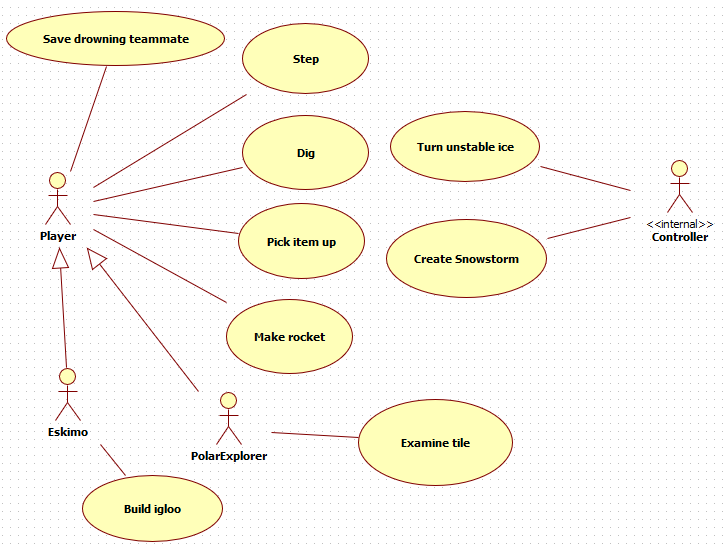
\includegraphics[width=17cm]{chapters/chapter02/use-case.png}
		\caption{Use-Case diagram}
		\label{fig:usecase}
	\end{center}
\end{figure}

\subsection{Use-case leírások}

%\comment{Minden use-case-hez külön}
% TODO: forgatókönyvek
\usecase{Step}{A játékos lép}{Player}{1. A játékos átlép egy másik jégtáblára. \newline 1.A A játékos telített instabil jégre lép, ami átfordul emiatt, a játékos vízbe esik. \newline 1.B A játékos lyukra lép, vízbe esik.}

% ez lehetne inkább Shovel
\usecase{Dig}{A játékos ás}{Player}{1. A játékos eltávolít egy réteg havat a jégmezőről. \newline 1.A A játékos két réteg havat távolít el a jégmezőről a lapátja segítségével.}

\usecase{Pick item up}{A játékos felvesz egy tárgyat}{Player}{1. A játékos felvesz egy tárgyat. \newline 2. A tárgy a játékos tárgyai közt helyet foglal. \newline 2.A A játékos ételt vesz fel, ami növeli a testhőjét.}

\usecase{Make rocket}{Játékos megkísérli a játékot megnyerő rakéta összerakását}{Player}{1.A játékos és csapattársai sikeresen összerakják a rakétát és megnyerik a játékot. \newline 1.A A játékos és csapattársai nem rendelkeznek a megfelelő alkatrészekkel, vagy nem állnak egymáshoz elég közel és a rakéta nem épül össze.}

\usecase{Save drowning teammate}{Játékos megmenti fulladozó csapattársát}{Player}{1. A játékos dob egy kötelet fulladozó társának, megmentve őt.}

\usecase{Build igloo}{Eszkimó játékos iglut épít}{Eskimo}{1. Egy kiválasztott jégtáblára iglut épít az eszkimó.}
\newpage
\usecase{Examine tile}{Sarkkutató játékos megnéz egy jégtáblát}{PolarExplorer}{1. Egy jégtábla teherbírását megnézi a sarkkutató}

\usecase{Turn unstable ice}{Túlterhelt, instabil jégtábla megfordul.}{Controller}{1. A túlterhelt jégtáblán lévő játékosok vízbe esnek \newline 2. A játékosok búvárruha vagy csapattárs segítsége miatt túlélik a vízbeesést. \newline 2.A Egy játékos nem éli túl a vízbe esést, a játék véget ér.}

\usecase{Create snowstorm}{Feltámad egy hóvihar}{Controller}{1. Egy hóvihar feltámad, ami néhány jégtáblán végigsöpör. \newline 2. A jégtáblákat hóval befedi, a játékosok testhőjét csökkenti a vihar.}
\newpage
\section{Szótár}
%\comment{A szótár a követelmények alapján készítendő fejezet. Egy szótári bejegyzés definiálásához csak más szótári bejegyzések és köznapi – a feladattól független – fogalmak használhatók fel. A szótár mérete kb. 1-2 oldal legyen.}

% TODO: szótár
\textbf{Alkatrész:} Jelzőrakéta összeszereléséhez szükséges tárgy. \\
\textbf{Átfordul (jégtábla):} Instabil jégtáblával történik, ha túl sokan  tartózkodnak rajta: A jégtáblán állók a vízbe esnek. \\
\textbf{Búvárruha:} Tárgy, túlélhető vele a vízbe esés. \\
\textbf{Elsütni (jelzőrakétát):} Tevékenység, jó esetben a játék megnyerése. \\
\textbf{Eltakarít (szereplő, havat):} Tevékenység, egy jégtábla hószintjének csökkentése. \\
\textbf{Építeni (iglut):} Tevékenység, iglu létrehozása. \\
\textbf{Eszkimó:} Osztály, képessége az iglu építés, kezdő testhője öt. \\
\textbf{Élelem:} Tárgy, testhő növelésére alkalmas. \\
\textbf{Fulladás:} Ha egy játékos a vízbe esik és nem segít rajta egy társa vagy nincs búvár ruhája, akkor megfullad (meghal). \\
\textbf{Felvesz (szereplő. tárgyat):} A szereplő egy tárgyat vagy elhelyez a saját tárgyai között. \\
\textbf{Hó:} Jégtábla tulajdonsága. \\
\textbf{Hóvihar:} Esemény, random következik be érinthet szereplőt vagy jégtáblát. \\
\textbf{Hóvihar elkap (jégtáblát):} A jégtáblát újra hó fedi be. \\
\textbf{Hóvihar elkap (szereplőt):} A szereplő testhője eggyel csökken. \\
\textbf{Iglu:} Játéktér eleme. Jégtáblán létezhet. Tartózkodhatnak benne szereplők. \\
\textbf{Instabil (jégtábla):} Olyan jégtáblák, amelyek átfordulnak, ha túl sokan vannak rajta. \\
\textbf{Játék:} Ez a szoftver. \\
\textbf{Jégmező:} A játéktér. \\
\textbf{Jégtábla:} A játéktér egy eleme. \\
\textbf{Jelzőfény:} Alkatrész a jelzőrakéta összerakásához. \\
\textbf{Jelzőrakéta:} Tárgy, a játék megnyeréséhez szükséges. \\
\textbf{Képesség:} Osztályra jellemző tevékenység. \\
%\textbf{Kiás (szereplő, tárgyat):} Tevékenység, \\
\textbf{Kimenekíteni (szereplő, szereplőt):} Kötél segítségével egy szereplő ki tud menekíteni egy másik vízbe esett szereplőt. \\
\textbf{Kör:} Időegység, minden körben minden szereplő 4 munkát végezhet. \\
\textbf{Kötél:} Tárgy, vízbe esett játékos megmenthető vele. \\
\textbf{Lapát:} Tárgy, eltakarítható vele a hó a jégtáblákról. \\
\textbf{Lép (szereplő jégtáblára):} Tevékenység, amivel egy szereplő változtatni tudja a helyzetét. \\
\textbf{Lyuk:} A játéktér eleme. Jégtáblán létezhet, ha egy szereplő rááll, akkor vízbe esik. \\
\textbf{Meghal (szereplő):} Az az összes testhő egység elvesztése vagy fulladás, következménye a játék elvesztése. \\
\textbf{Megnézni (jégtáblát):} Sarkkutató képessége, megállapítja egy jégtábla teherbírását.
\textbf{Munka:} Egy szereplő által, egy körben végezhető tevékenységek száma. \\
\textbf{Osztály:} Szereplő fajta. \\
\textbf{Összeszerelni (jelzőrakétát):} Ha a szereplők megtalálják az összes alkatrészt és ugyan arra a jégtáblára helyezik őket, akkor hajthatják végre ezt a tevékenységet. \\
\textbf{Patron:} Alkatrész a jelzőrakéta összerakásához. \\
\textbf{Pisztoly:} Alkatrész  a jelzőrakéta összerakásához.\\
\textbf{Sarkkutató:} Osztály, képessége a jégtábla megnézése, kezdő testhője négy. \\
\textbf{Stabil (jégtábla):} Olyan jégtábla, amelyen akárhány szereplő állhat. \\
\textbf{Szereplő:} Egy játékos avatárja a játéktéren. \\
\textbf{Tárgy:} Entitás, létezhet jégtáblába fagyva, vagy szereplő birtokában. \\
\textbf{Tenger:} A játéktér eleme, körülveszi a jégmezőt. \\
\textbf{Tesszaláció:} Kétdimenziós síkon egy geometriai forma ismétlése átlapolás és rések nélkül.
\textbf{Testhő:} Szereplő tulajdonsága, ha elfogy akkor meghal. \\
\textbf{Tevékenység:} Egy szereplő megváltoztatja a játékteret. \\
\textbf{Tiszta (jégtábla):} Jégtábla, amin nincs hó. \\
\textbf{Vízbe esik (szereplő):} Akkor következhet be, ha az adott szereplő lyukra áll vagy átfordul alatta a jégtábla \\
\newpage


\section{Projekt terv}
%\comment{Tartalmaznia kell a projekt végrehajtásának lépéseit, a lépések, eredmények határidejét, az egyes feladatok elvégzéséért felelős személyek nevét és beosztását, a szükséges erőforrásokat, stb. Meg kell adni a csoportmunkát támogató eszközöket, a választott technikákat! Definiálni kell, hogy hogyan történik a dokumentumok és a forráskód megosztása!}
% TODO: projekt terv
\subsection{Végrehajtás lépései}
	\begin{tabular}{|l|l|}
		\hline
		febr. 24. & Követelmény, projekt, funkcionalitás dokumentum elkészítése                                            \\ \hline
		márc. 2.  & Analízis modell kidolgozása 1                                                                          \\ \hline
		márc. 9.  & Analízis modell kidolgozása 2                                                                          \\ \hline
		márc. 16. & Szkeleton tervezése                                                                                    \\ \hline
		márc. 23. & Szkeleton - beadás és a forráskód herculesre való feltöltése                                           \\ \hline
		márc. 30. & Prototípus koncepciójának elkészítése                                                                  \\ \hline
		ápr. 6.   & Részletes tervek elkészítése                                                                           \\ \hline
		ápr. 20.  & Prototípus készítése, tesztelése                                                                       \\ \hline
		ápr. 27.  & Prototípus - beadás és a forráskód, a tesztbemenetek és az elvárt kimenetek herculesre való feltöltése \\ \hline
		máj. 4.   & Grafikus felület specifikációja                                                                        \\ \hline
		máj. 18.  & Grafikus változat és Összefoglalás - beadás és a forráskód herculesre való feltöltése                  \\ \hline
	\end{tabular}

\subsection{Beosztás}
Minden héten az aheti feladattal a csapat összes tagja dolgozni fog, különböző mértékben, ahogy a tagok ideje engedi. Az 5 fős csapat összetartásáért, és hogy elkészüljön a feladat a csapat vezetője, Kiss Andor a felelős. A dokumentumok nyomtatásáért minden héten beadás előtt megbeszéljük a felelőst. Az UML-es részekkel főleg Kiss Andor, a grafikával főleg Máté Botond tervez majd foglalkozni, de mindenki más is kiveszi a részét a dologból.

\subsection{Erőforrások:}
A tagok közti kommunikációt egy Facebook Messengeres beszélgetős csoportban csináljuk főleg, emellett persze előjöhet a projekt labor feladatainak témája amikor élőben találkozunk, akkor is, például előadáson, konzultáción, vagy egy közeli sörözőben.
A verziókezeléshez Git-et használunk, a fájlok és a tervek megosztásához Github-ot és Google Docs-ot használunk.
A dokumentációhoz LaTeX-et és Microsoft Wordöt használunk.
Modellezéshez WhiteStarUML-t használunk.
Fejlesztőkörnyezetként IntelliJ-t vagy Eclipset használunk, ez a tagok egyéni preferenciája.
Fordításoz a fejlesztőkörnyezetet használjuk.


% vázlat:
% 	- lépések, határidők: https://www.iit.bme.hu/targyak/BMEVIIIAB02/%C3%BCtemterv-hat%C3%A1rid%C5%91k
%		- követelmény, projekt, funkcionalitás: 2020. febr. 24.
%		- analízis modell: 2020. márc. 9.
%		- szkeleton: 2020. márc. 23.
%		- prototípus: 2020. ápr. 20.
%		- grafikus release: 2020. máj. 18.
%	- beosztások
%		- andor: nem szeret grafikázni, szeret umlezni
%		- márk: ?
%		- balázs: ?
%		- boti: szeret grafikázni
%		- gábor: ?
%	- ezközök
%		- facebook messenger (discord?)
%		- github
%		- latex
%		- whitestaruml
%		- fejlesztőkörnyezet: intellij? eclipse?
%		- build system: gnu make?
%		- google drive?, docs?


